\section{Introduction}
Das ist der Einleitungsteil unserer Hausarbeit, die bei weitem noch nicht fertig ist.

\subsection{Research question}
Kleiner Reminder für mich in Bezug auf die Dinge, die wir bei der Thesis beachten sollten und \LaTeX{}-Vorlage für die Thesis.

\subsection{Research objective}
chapter \ref{infos} enthält die Inhalte des Thesis-Days und alles, was zum inhaltlichen erstellen der Thesis relevant sein könnte. In chapter \ref{latexDetails} \nameref{latexDetails} findet ihr wichtige Anmerkungen zu \LaTeX{}, wobei die wirklich wichtigen Dinge im Quelltext dieses Dokumentes stehen (siehe auch die Verzeichnisstruktur in Abbildung \ref{fig:verzeichnisStruktur}).

\subsection{Motivation for researching WASM}
Die Motivation dieser Studie liegt darin, die Leistungsfähigkeit von WebAssembly im Vergleich zu JavaScript zu untersuchen, zu klarifizieren und zu bewerten. Die daraus resultierenden Ergebnisse sind vorallem deshalb interessant, da dieser Webstandard im Vergleich zu JavaScript relativ neu ist.
Aus diesem Grund ist es unserer Meinung nach wichtig, diesen Standard weiter tiefgründig zu erforschen, um eine sinnvolle Nutzung und eingehende Weiterentwicklungen möglich zu machen. Darüber hinaus möchten wir ein tieferes Verständnis für die Leistungseigenschaften von WebAssembly im Vergleich zu JavaScript ergründen. Dazu sind sowohl Recherchen über bereits vorhandene Analysen als auch eine eigenständige Analyse zu den beiden Webstandards sinnvoll und notwendig.
Insgesamt, möchten wir mit dieser Arbeit im Rahmen einer umfassenden Analyse, einen Beitrag zur Performance-Debatte zwischen WebAssembly und JavaScript leisten.

\begin{figure}[H]
\caption{Verzeichnisstruktur der \LaTeX{}-Datein}\label{fig:verzeichnisStruktur}
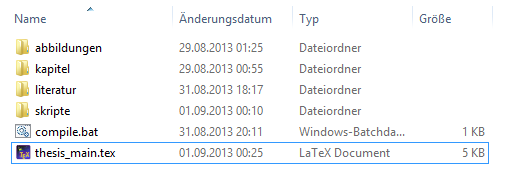
\includegraphics[width=0.9\textwidth]{verzeichnisStruktur}
\\
Quelle: Eigene Darstellung
\end{figure}
